\documentclass[]{standalone} 
\usepackage{pgfplots} 
%\usepgfplotslibrary{external} 
%\tikzexternalize 
\usepgfplotslibrary{fillbetween}
\usepackage{tikz} 
\usepackage{amsmath} 
\usepackage{pgfplots} 
\usetikzlibrary{calc} 
\pgfplotsset{compat = newest, every axis plot post/.style={line join=round}, label style={font=\Large} }
\begin{document} 
	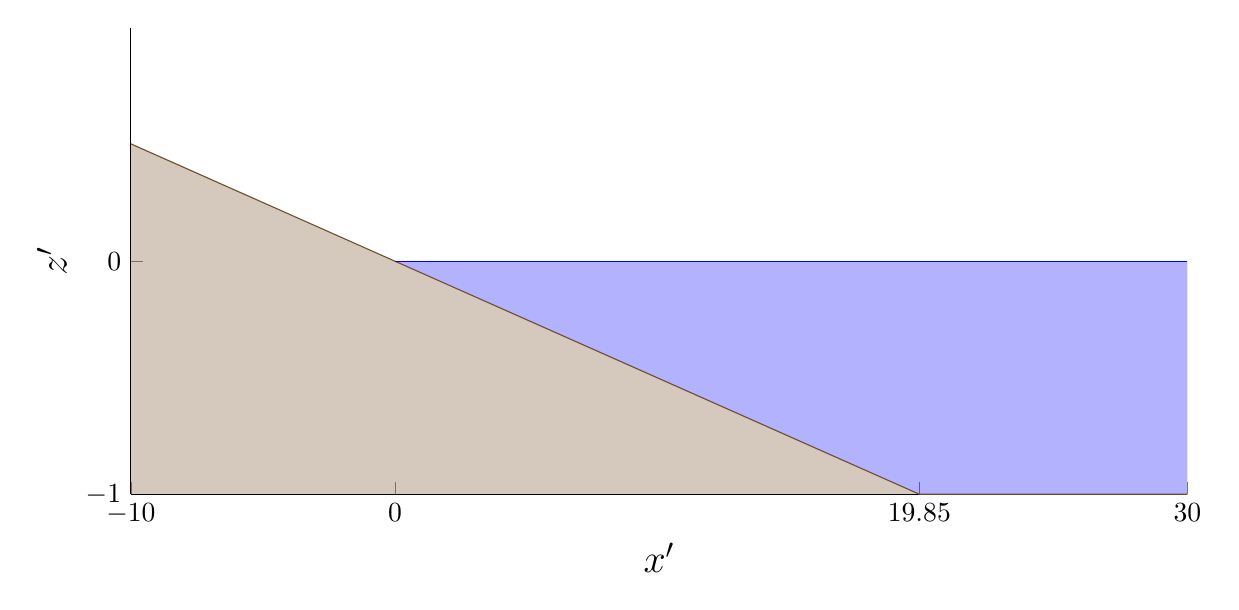
\begin{tikzpicture}
	\begin{axis}[ 
	width = 0.7\textwidth,
	width=15cm,
	height = 7.5cm,
	axis y line*=left,
	axis x line*=bottom, 
	xtick={0,19.85,-10,30},  
	ytick = {0,-1}, 
	xmin=-10, 
	xmax=30, 
	ymin =-1, 
	ymax = 1,
	xlabel=$x'$, 
	ylabel=$z'$]
	
	\addplot [name path=b,brown!60!black] coordinates {(30,-1) (19.85,-1)  (0,0) (-19.85,1)};
	
	\path[name path=axis] (axis cs:-10,-1) -- (axis cs:30,-1);
	
	\addplot [name path=a,blue] coordinates {(0,0.0) (30,0)};
	
		\addplot [
		thick,
		color=brown!60!black,
		fill=brown!60!black, 
		fill opacity=0.3
		] fill between[of=b and axis];
		
	\addplot [
	thick,
	color=blue,
	fill=blue, 
	fill opacity=0.3
	] fill between[of=a and b];
	

	\end{axis} 
	
	
	
	\end{tikzpicture}
\end{document}